% \documentclass[twocolumn]{article}
\documentclass[]{article}
\usepackage[utf8]{inputenc}
\usepackage{amsmath}
\usepackage{authblk}
\usepackage{graphicx}
\usepackage{caption}
\usepackage{subcaption}
\usepackage[english]{babel}
\usepackage{csquotes}
% \usepackage{multicol}
\usepackage{cuted}
\usepackage{listings}
\usepackage[section]{placeins}

\lstset{
  basicstyle=\ttfamily,
  columns=fullflexible,
%   frame=single,
  breaklines=true
}

\usepackage[acronym]{glossaries}
\newacronym{ros}{ROS}{Robot Operating System}
\newacronym{slam}{SLAM}{Simultaneous Localization and Mapping}

\usepackage[sorting=none]{biblatex}
\addbibresource{bib.bib}

\usepackage[dvipsnames]{xcolor}
\newcommand{\TODO}[1]{\colorbox{Red}{TODO #1}}

\title{MIR Cleaner - an autonomous mapping and vacuum platform}
\author[1]{João Santos, 76912}
\affil[1]{Department of Electronics, Telecommunications and Informatics, University of Aveiro}
\date{July 2022}

\begin{document}

\maketitle

\section{Introduction}

One of the key responsibilities of each and every person is keeping the environment around us clean.

With their cutting-edge technologies, robots are playing a significant role in modern society and improving the quality of human life. The floor-cleaning robots are useful in households where they can substitute humans.

Fundamentally, the robot vacuum cleaners have stood out for their abilities. Some currently available products are based on the basic obstacle avoidance (employing infrared or ultrasonic sensors), while others use laser mapping technologies.

Each cleaning system has unique benefits and drawbacks. For instance, some of the robots that use laser mapping are considerably quicker, more energy-efficient but also more expensive. In contrast, due to their random cleaning, obstacle avoidance-based vacuum robots require more time and energy but are less expensive.

In this assignment, a new approach was implemented based on exploration and planning techniques, based on the MIR100 mobile base.

\section{Installation}

The base framework for this assignment was the \gls{ros} Noetic Ninjemys and so it should be already installed. Additionally, Gazebo must also be installed. Rviz is also needed so the cleaning agent can be started and it also is helpful for visualization.

On top of the previous software, some \gls{ros} packages are also needed that have not been developed by the author. They are:
%
\begin{itemize}
    \item \textit{mir\_gazebo}
    \item \textit{mir\_naviagtion}
    \item \textit{ira\_laser\_tools}
    \item \textit{move\_base}
    \item \textit{gmapping}
    \item \textit{explore\_lite}
    \item \textit{amcl}
    \item \textit{map\_server}
    \item \textit{costmap\_2d}
\end{itemize}

To install them, use the following bash script:
%
\begin{lstlisting}[language=bash]
    #!/bin/bash
    sudo apt install ros-noetic-mir-gazebo
    sudo apt install ros-noetic-mir-navigation
    sudo apt install ros-noetic-ira-laser-tools
    sudo apt install ros-noetic-move-base
    sudo apt install ros-noetic-gmapping
    sudo apt install ros-noetic-explore-lite
    sudo apt install ros-noetic-amcl
    sudo apt install ros-noetic-map-server
    sudo apt install ros-noetic-costmap-2d
\end{lstlisting}
%
The final external package needed is rm\_mir\_cleaner, that must be inside the \textit{src} folder of the \gls{ros} workspace, can be obtained by:
%
\begin{lstlisting}[language=bash]
    git clone git@github.com:nunolau/rm_mir_cleaner.git
\end{lstlisting}

Then, just add this package\footnote{\url{https://github.com/joao-pm-santos96/rm_cleaner_76912}} to the mentioned \textit{src} folder and build the workspace using \textit{catkin build}.


\section{Usage}

The developed package is composed by multiple launch files. The base launch file (which is requested for both the exploration and cleaning agents) is \textit{bringup.launch}.

This launch file is responsible for launching two fundamental nodes: laserscan\_multi\_merger and move\_base. laserscan\_multi\_merger is a node from ira\_laser\_tools that listens from both laser scanners of the MIR100 robot and publishes a combined laser scan message. 

The move\_base node deals with the navigation stack of the robot, namely, the local and global costmaps and planners.

Four arguments can be set:

\begin{description}
    \item[rviz] Set to \textit{true} to launch a pre-configured Rviz instance. Default is \textit{false}.
    \item[unpause] Set to \textit{true} to unpause Gazebo. Default is \textit{false}.
    \item[map] Load pre-defined maps. Set \textit{0} for \textit{mir\_empty\_world} with \textit{rm\_mir\_cleaner} simple model, or \textit{1} for \textit{mir\_maze\_world} from \textit{mir\_gazebo}. Default is \textit{-1} (no map).
    \item[gui] used together with \textbf{map}. If \textit{true}, Gazebo GUI is launched. Default is \textit{false}.
\end{description}

The \textbf{map} argument will launch the described maps. Yet, other maps may be launched externally and used with this package. Is this is the case, keep this argument to the default value.

\subsection{Exploring agent}

To perform the exploration of a unknown environment, the \textit{explore.launch} file is used. This launch file launches \textit{gmapping} and \textit{explore\_lite}.

To start the exploring agent in the default map 1 and with Rviz, run (in separate terminals)
%
\begin{lstlisting}[language=bash]
    roslaunch rm_cleaner_76912 bringup.launch gui:=false map:=1 unpause:=true rviz:=true
    roslaunch rm_cleaner_76912 explore.launch
\end{lstlisting}
%
and then you should visualize something like Fig. \ref{fig:explore_agent}.

\begin{figure}[ht]
    \centering
    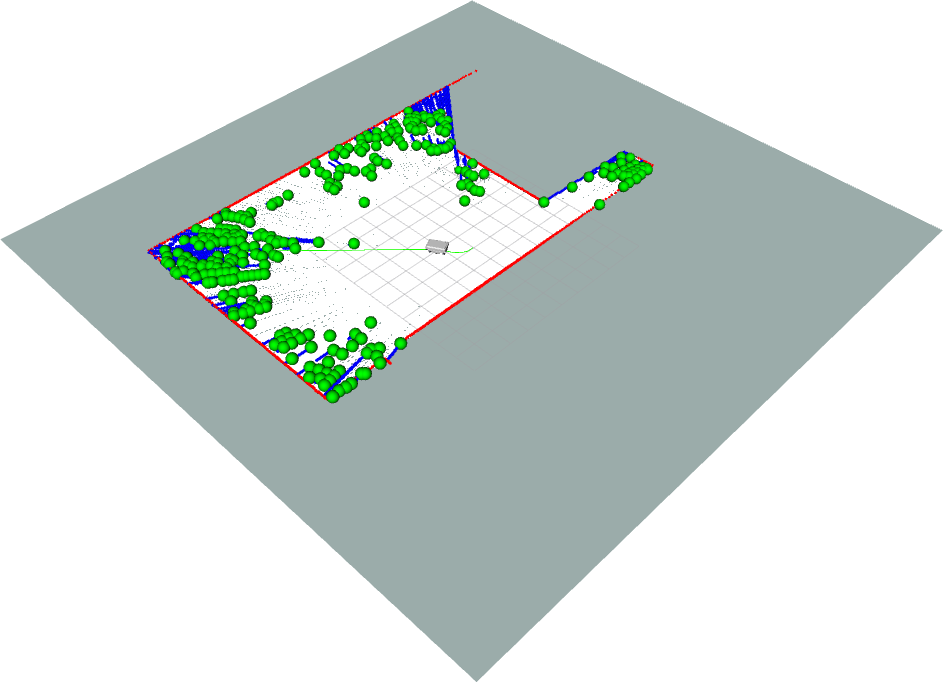
\includegraphics[width=0.8\textwidth]{imgs/explore_agent.png}
    \caption{Exploration agent on default map 1.}
    \label{fig:explore_agent}
\end{figure}

In the end, when the exploration ends, you may save the map by running 
%
\begin{lstlisting}[language=bash]
    roslaunch rm_cleaner_76912 map_save.launch map_name:=<map_name>
\end{lstlisting}
%
which will save the current map to the default folder (the \textit{maps} folder on the package root) with the \textless map\_name\textgreater.yaml name. 

\subsection{Cleaning agent}

Now that the environment is known, the agent is able to vacuum it. For that, \textit{clean.launch} must be started. 

This file has two arguments
%
\begin{description}
    \item[map\_file] the path to the map the agent has already created. It must be the full path and end with the file extension (.yaml).
    \item[clean\_goal] the ratio of the environment to be cleaned, in the range of 0.0 to 1.0.
\end{description}
%
and will launch four nodes: \textit{amcl}, \textit{map\_server}, \textit{costmap\_2d} and \textit{cleaner\_bot.py}.

Continuing the previous example, run (in separate terminals)
%
\begin{lstlisting}[language=bash]
    roslaunch rm_cleaner_76912 bringup.launch gui:=false map:=1 unpause:=true rviz:=true
    roslaunch rm_cleaner_76912 clean.launch map_file:=/home/<user_name>/rm_cleaner_ws/src/rm_cleaner_76912/maps/<map_name>.yaml clean_goal:=<goal>
\end{lstlisting}
%
after which, something similar to Fig. \ref{fig:clean_agent} should appear.

\begin{figure}[ht]
    \centering
    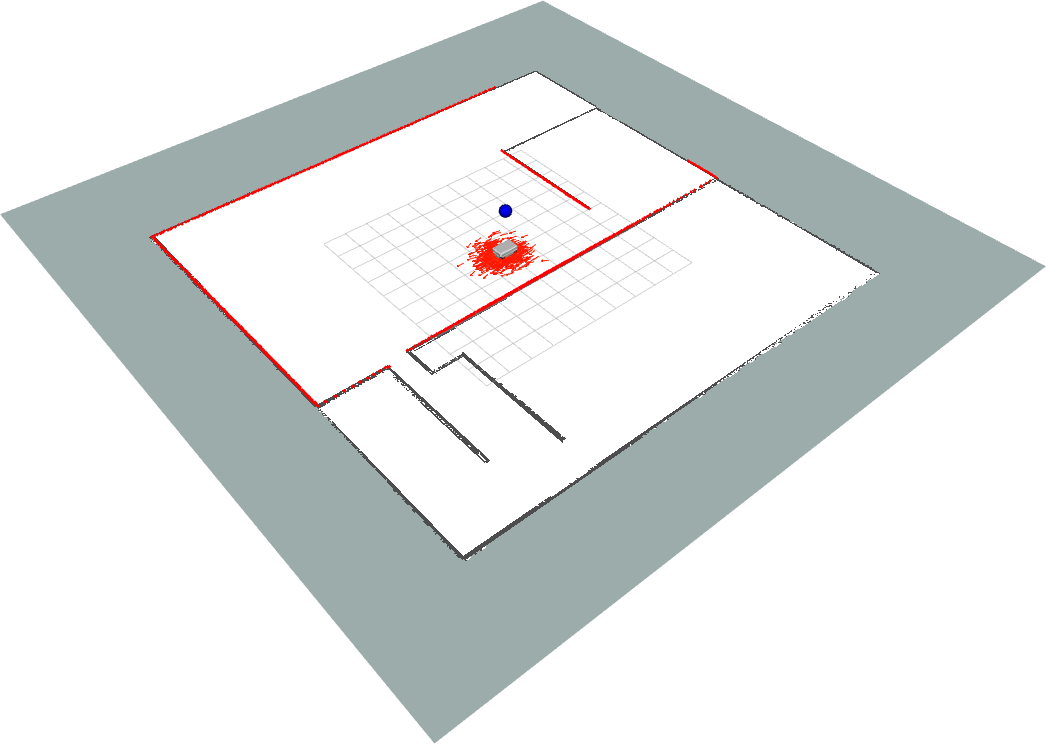
\includegraphics[width=0.8\textwidth]{imgs/clean_agent.png}
    \caption{Cleaning agent on default map 1.}
    \label{fig:clean_agent}
\end{figure}

To start the cleaning behaviour, press the blue marker (see Fig. \ref{fig:clean_agent}) on Rviz. This will instruct the robot to perform the computed path until it cleans at least the desired ratio or the path is concluded (in which case, it is assumed that all the accessible space has been cleaned).

Notice that, because \textit{amcl} is being used for the cleaning agent, a start pose is required. By default, \textit{amcl} expects the robot to be at the origin of the map, and within a $5 \times 5 \text{ m}^2$ area. If this is not the case, please provide an approximated pose through the Rviz GUI or a published message.

\section{Methodology}

The adopted methodology consists in two distinct agents. One that will explore the environment, and another that will vacuum it.

Their implementations are discussed in the following sections.

\subsection{Exploration and map building}

The exploration agent is based is two well-known packages: \textit{gmapping} and\textit{explore\_lite}. Combined, they are able to autonomously navigate through unknown spaces, maintaining a probabilistic localization within it and recording both the free and occupied spaces already encountered.

\subsubsection{SLAM}

The \textit{gmapping} \cite{grisetti2005improving, grisetti2007improved} package provides laser-based \gls{slam}, enabling the creation of a 2D occupancy grid based on the laser data and pose of the robot.

This package implements a Rao-Blackwellized particle filter as an effective mean to solve the \gls{slam} problem. This method makes use of a particle filter where each particle carries its own map of the surrounding area.

\subsubsection{Exploration}

In parallel, the \textit{explore\_lite} \cite{Horner2016} package provides greedy frontier-based exploration, which will instruct (through the \textit{move\_base} node) the robot to greedily explore the environment until no frontiers can be found. This behaviour is illustrated on Fig. \ref{fig:exploration_step}.

\begin{figure}[ht]
    \centering
    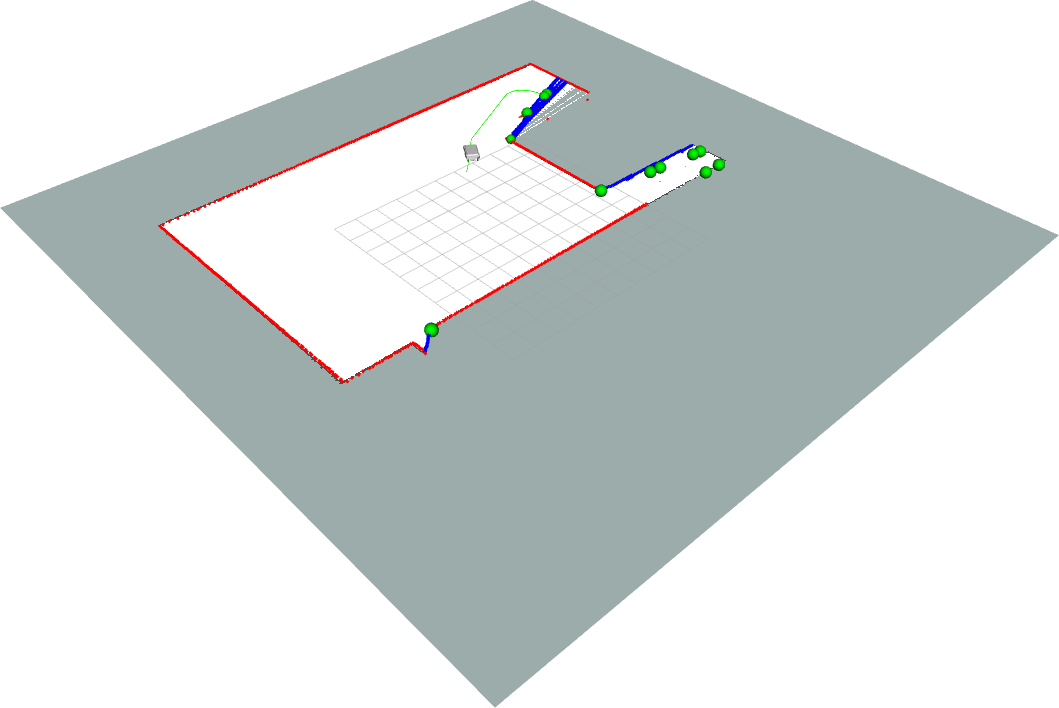
\includegraphics[width=0.8\textwidth]{imgs/exploration_step.png}
    \caption{Exploration step. The robot will follow the path (green line) to try to see through the next frontier (blue lines).}
    \label{fig:exploration_step}
\end{figure}

Frontiers are regions on the border between open space and unexplored space. The robot can view into unmapped space from any frontier and add the new discoveries to its map, which may include some new frontiers. This way, the agent can create a map of all locations that are able to be reached in the environment by exploring each frontier or determining that it is inaccessible.

\subsection{Cleaning}

The cleaning agent has, \textit{a priori}, the knowledge of the map it is required to clean. This is an advantage, allowing the agent to plan the path to transverse. The challenge here is then to compute a full coverage path, i.e., a path that allows the clean bar (mounted in front of the MIR100) to be moved across all space.

\subsubsection{Vacuum area}

The agent is requested to clean (i.e. transverse) a given ratio of all free space in the known map. To compute this ratio, the agent must know the space that it is free to visit and the space that it has already vacuumed. 

The information about the the free space is encoded in the provided map and, thus, trivial to obtain.

On the other hand, there are some challenges on tracking the cleaned area. For example, if the robot visits the same area multiple times, the ratio of cleaned space must not change. The implemented solution is based on an extra occupancy grid (not managed by the \textit{move\_base} node) that, at the start, marks all cells as unknown. The trick is that the cells in this occupancy grid (from now on, called cleaned area map) are marked as free if and only if they are run across by the cleaning bar. This behaviour is shown in Fig. \ref{fig:clean_bar_mapping}.

\begin{figure}[ht]
    \centering
    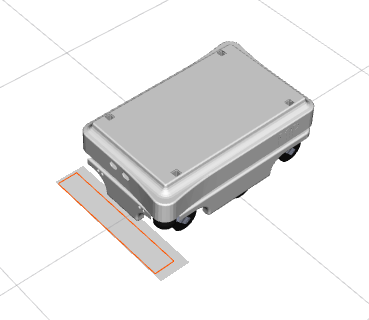
\includegraphics[width=0.8\textwidth]{imgs/clean_bar_mapping.png}
    \caption{Detailed demonstration of the virtual clean bar (in red) and the area marked as cleaned (in gray).}
    \label{fig:clean_bar_mapping}
\end{figure}

With this information, the agent is able to compute both the free and cleaned areas and then, the ratio of the known area cleaned.

\subsubsection{Localization}

In contrast to the exploration agent, \gls{slam} is not required. The localization process is done through a probabilistic localization system, the \textit{amcl} package. It employs the adaptive Monte Carlo localization technique, which compares the pose of the robot to a known map using a particle filter (see Fig. \ref{fig:amcl_init}).

\begin{figure}[ht]
    \centering
    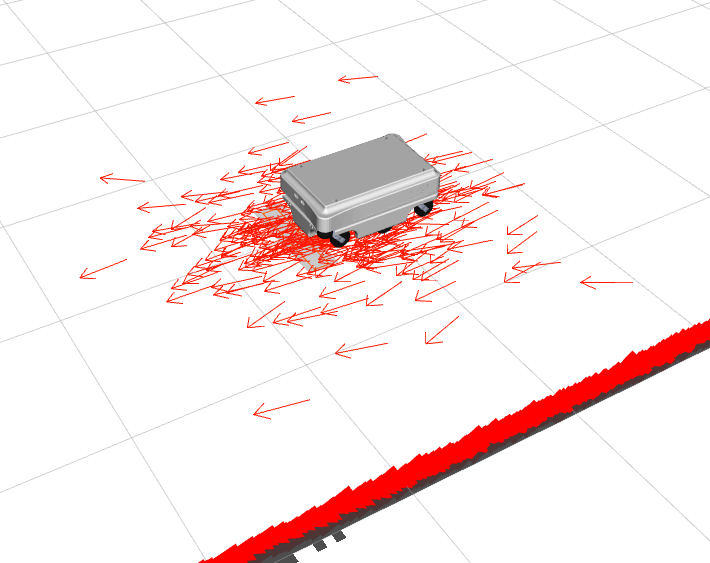
\includegraphics[width=0.8\textwidth]{imgs/amcl_init.png}
    \caption{Set of possible initial poses computed by \textit{amcl}.}
    \label{fig:amcl_init}
\end{figure}

\subsubsection{Path planning}

As previously mentioned, knowing the map is a big advantage for the agent, allowing it to plan a path. The implemented strategy consists in a \textit{zig-zag} motion. For this, the agent computes a set of poses that then are sent to the \textit{move\_base} node which, in turn, will move the robot. 

\begin{figure}[ht]
    \centering
    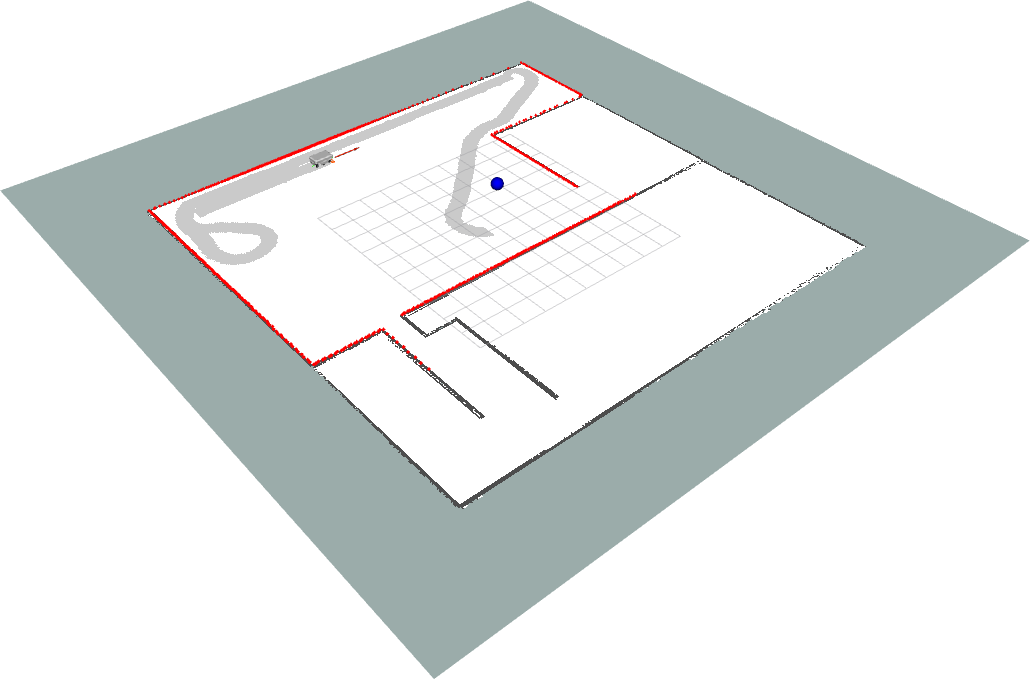
\includegraphics[width=0.8\textwidth]{imgs/cleanned_0.0756.png}
    \caption{Example step of the cleaning path (already covered 7.56\%).}
    \label{fig:cleaning_path}
\end{figure}

\section{Results}

The main take away from this assignment was the successful implementation of an autonomous exploring and cleaning agents. In this section, the results regard the harder map scenario (argument \textbf{map}:=1).

In Fig. \ref{fig:map1} the output map is shown. It is visible that the majority of the walls are completely reconstructed, apart from the upper left corner where some gaps exist. Yet, these gaps are not an issue to the current implementation given that they are severely smaller than the robot.

\begin{figure}[ht]
    \centering
    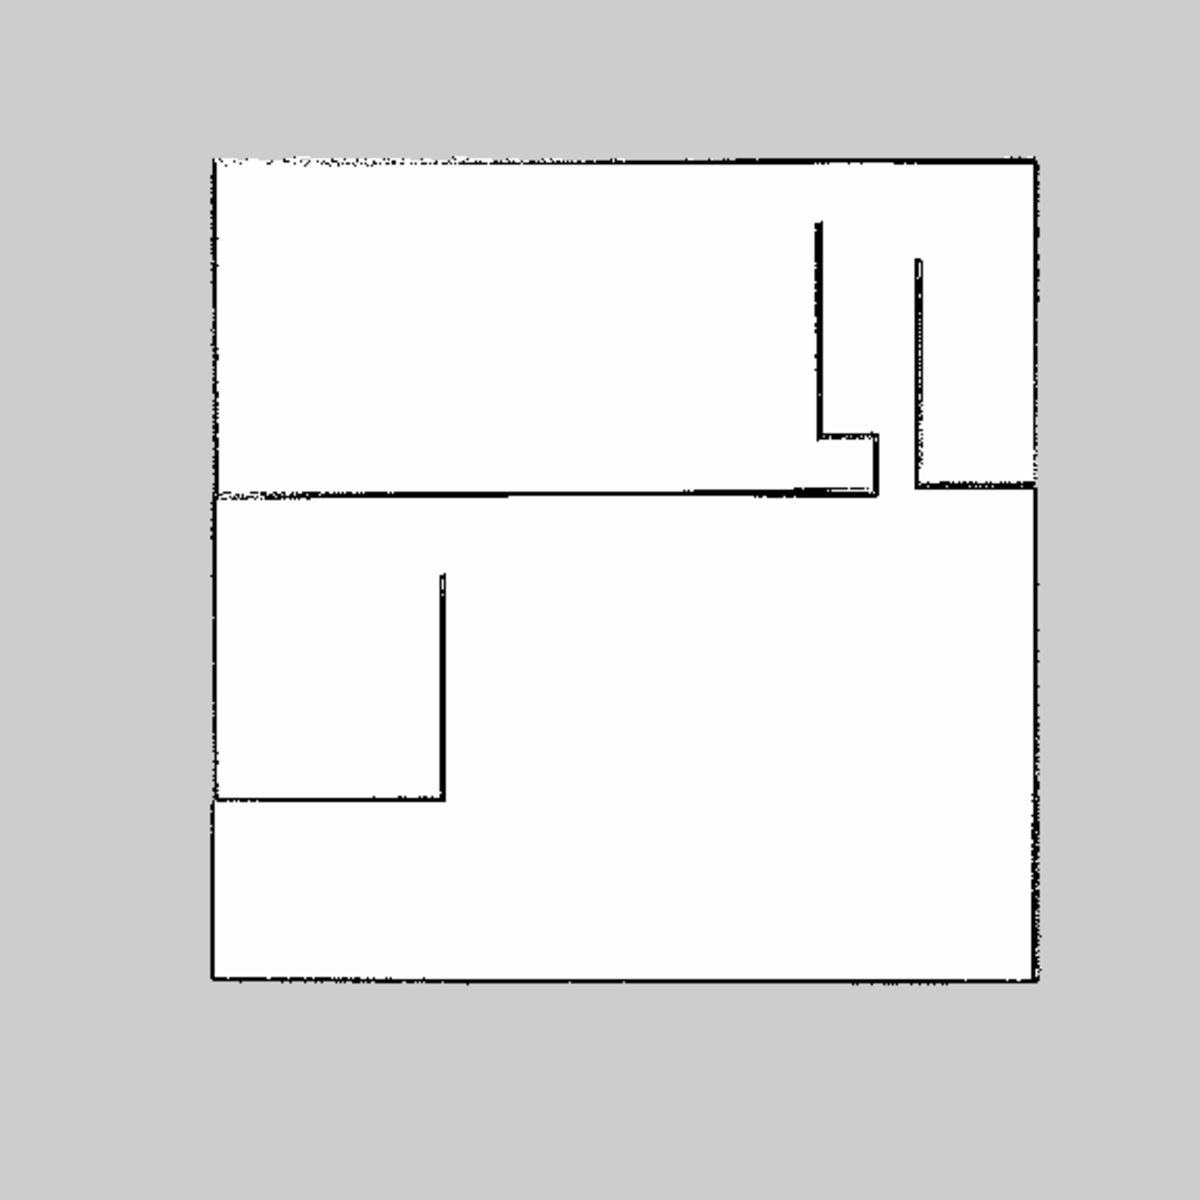
\includegraphics[width=0.8\textwidth]{imgs/map1.pdf}
    \caption{Output map autonomously created by the agent.}
    \label{fig:map1}
\end{figure}

Using the previous map, the agent performs a cleaning pattern as shown on Fig. \ref{fig:map1_cleaned}. In this scenario, 80\% of all free (an potentially reachable) space was vacuumed. 

\begin{figure}[ht]
    \centering
    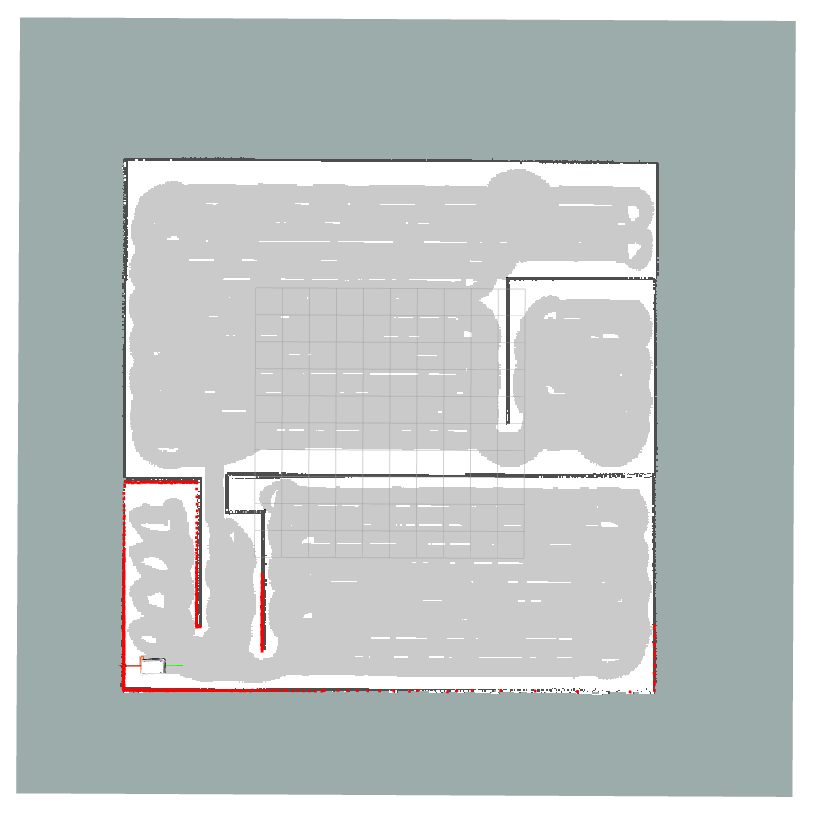
\includegraphics[width=0.8\textwidth]{imgs/map1_cleaned.png}
    \caption{Area autonomously cleaned by the agent (80\% of all free space).}
    \label{fig:map1_cleaned}
\end{figure}

A video of the behaviour is also available\footnote{\url{https://youtu.be/nQXJgW4vZ0M}}.

\subsection{Future work}

In a future development of this work, a better path planning methodology should be adopted. Namely, there are two aspects that can be greatly improved.

First, in the implemented agent, the next goal pose is sent to the \textit{move\_base} node when the last one is reached. Yet, the last one is only considered as reached when the robot stops within a certain tolerance. The stop of the motion creates an uneven motion. A better approach would be to implement a set of \gls{ros} planners (a global and a local) as plugins. In fact, a full path global planner already exists\footnote{see \url{http://wiki.ros.org/full_coverage_path_planner}} but none of the available local planners would follow it.

Secondly, the agent tries to move from one side of the map to another, in the \textit{zig-zag} motion, regardless if there is a wall in the middle or not, is the global planner can produce a path to the pose, then it will move there. This may not be the most efficient solution for a vacuum robot. A better solution would be to perform a cell decomposition on the known map and only then, apply this motion within each cell. This would create a more efficient cleaning pattern and would avoid the motion of the robot across the same path, multiple times.

\section{Conclusion}

The implemented agents reach both proposed goals, to explore unknown environments and to coverage them using the map, autonomously. This is, by itself, a success. Nonetheless some improvements could be made to to both the motion of the agent and the cleaning behaviour.

% \FloatBarrier
\printbibliography

\end{document}
